\begin{appendices}
    % Appendix titles modifyers
    \renewcommand{\theHchapter}{A\arabic{chapter}}
    \renewcommand{\theHsection}{A\arabic{section}}
    \renewcommand*{\justifyheading}{\raggedleft}
    \titleformat{\chapter}[display]
        {\vspace{-3cm}
            \normalfont\Huge\bfseries\justifyheading}
        {\color{gray} \fontsize{48}{48}\selectfont \appendixname 
        \hspace{0.1cm} \thechapter}
        {20pt}{\fontsize{48}{48}\selectfont}
    \titleformat{\section}
        {\normalfont\Large\bfseries}{\thesection}{1em}{}
    \titleformat{\subsection}
        {\normalfont\large\bfseries}{\thesubsection}{1em}{}
    \chapter{Manual de Usuario}
        En este anexo se facilitará un guía para el usuario. El propósito de esta guía es explicar al usuario cuáles son las capacidades de la aplicación y su modo de uso.
        \section{Registro}
        Para poder utilizar la aplicación el usuario deberá realizar primero el registro en el sistema. Este se realizará pulsando el botón de ``¿No tienes una cuenta? Regístrate''.
        
        Posteriormente el usuario procederá a rellenar la información que ahí se le pide como nombre, correo electrónico y contraseña que mínimo deberá ser de 6 caracteres.
        En el siguiente paso deberá rellenar datos como nombre de usuario y localización preferida a través de un mapa interactivo, asimismo como aceptar los términos y condiciones.

        Finalmente, para terminar el proceso de registro el usuario deberá confirmar su correo electrónico a través del enlace que le será enviado al buzón del correo electrónico especificado durante el registro.
    \begin{figure}[H]
    \centering
    \begin{minipage}{0.3\textwidth}
        \centering
        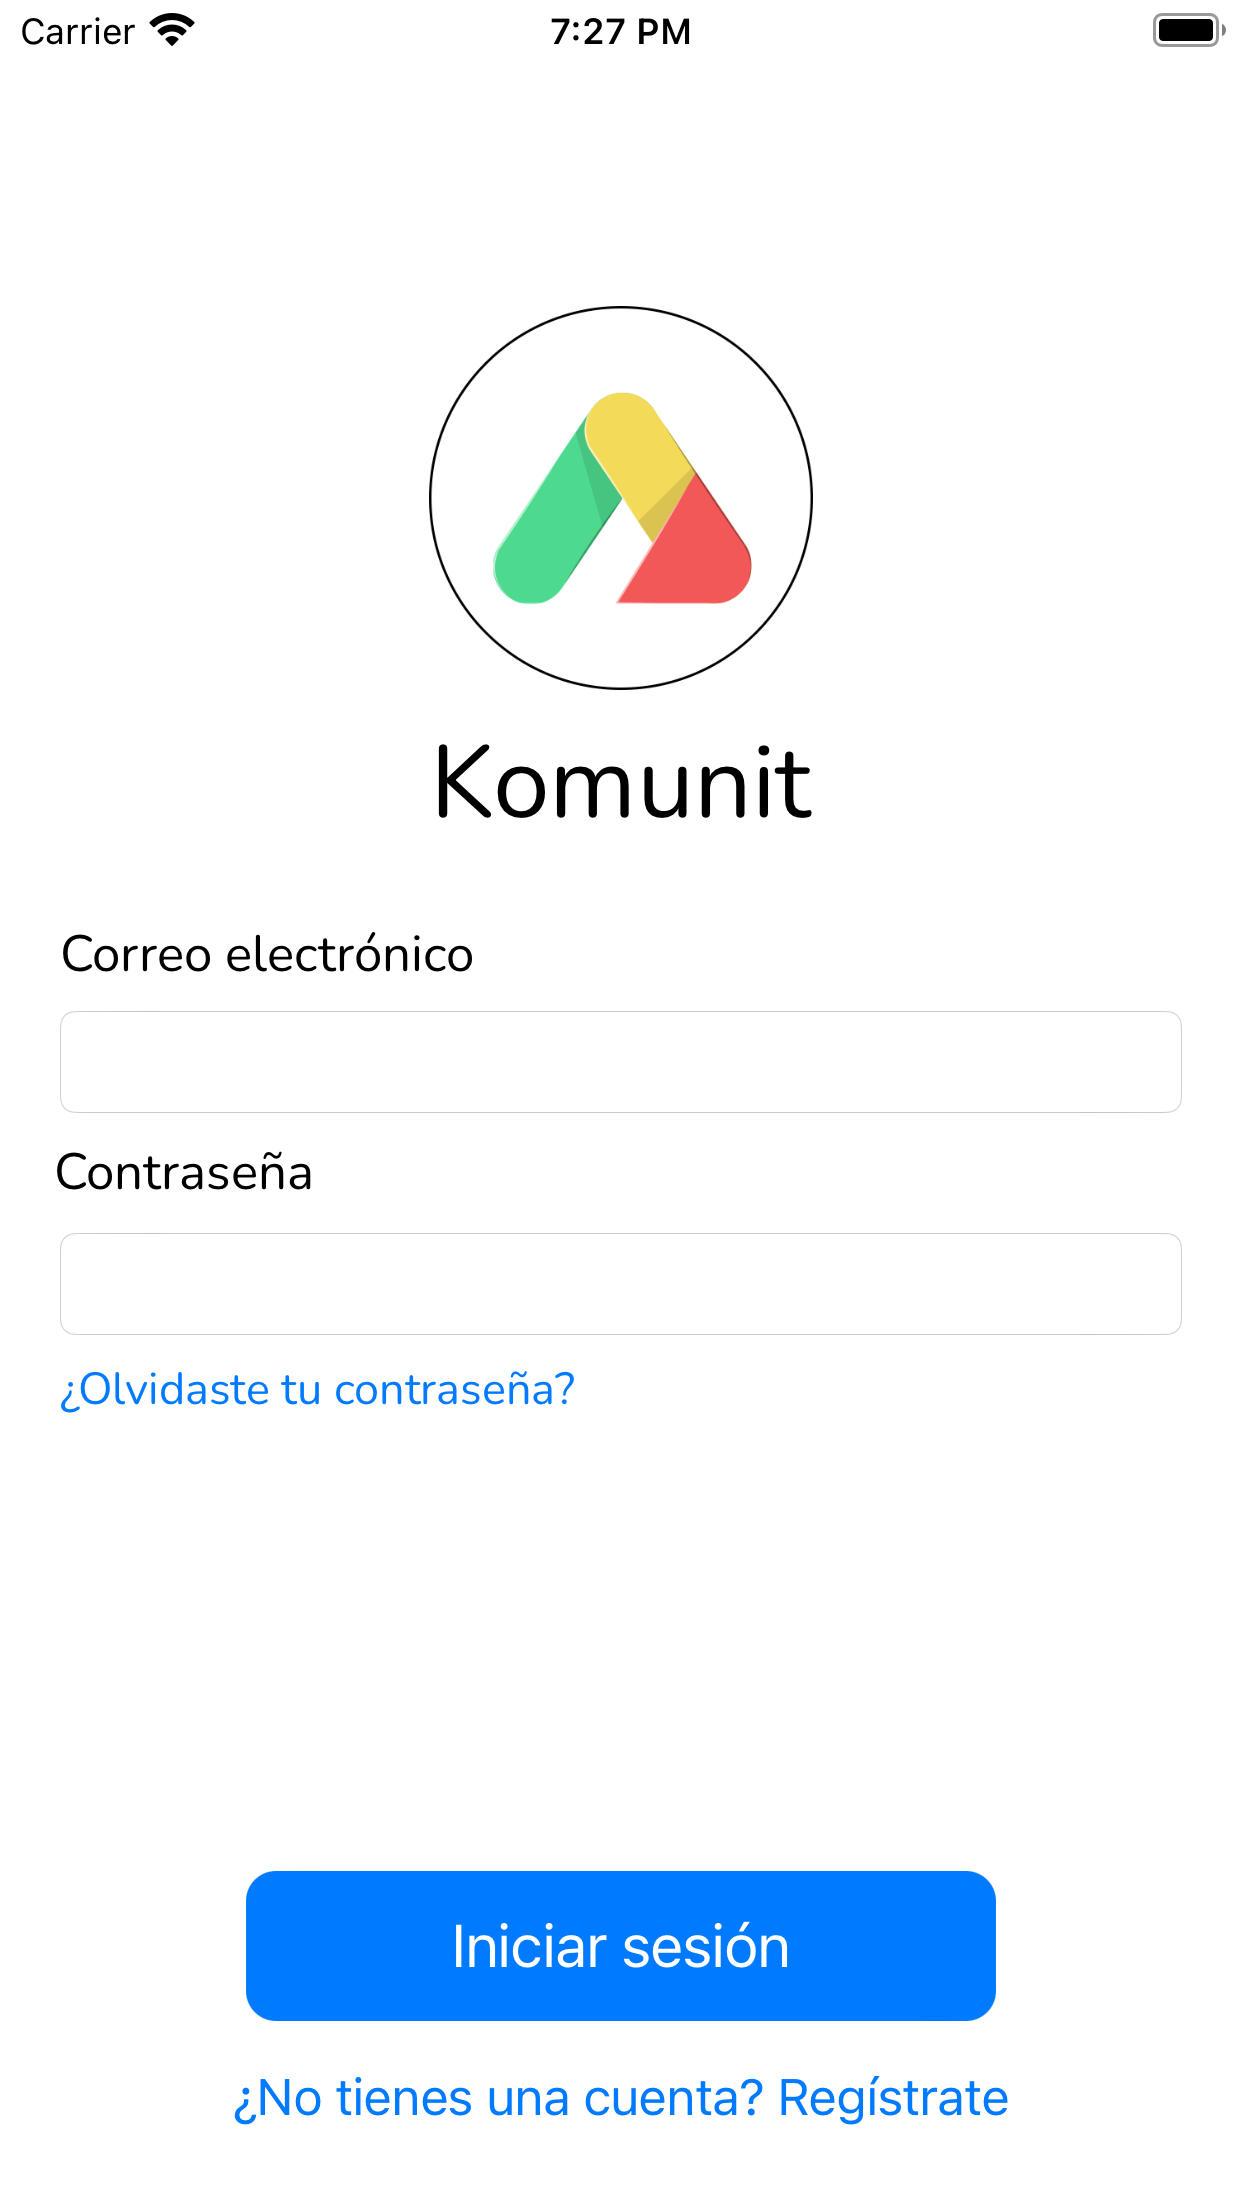
\includegraphics[cframe=black 2pt, width=1\linewidth]{images/manual/login.png}
    \end{minipage}
    \begin{minipage}{0.3\textwidth}
        \centering
        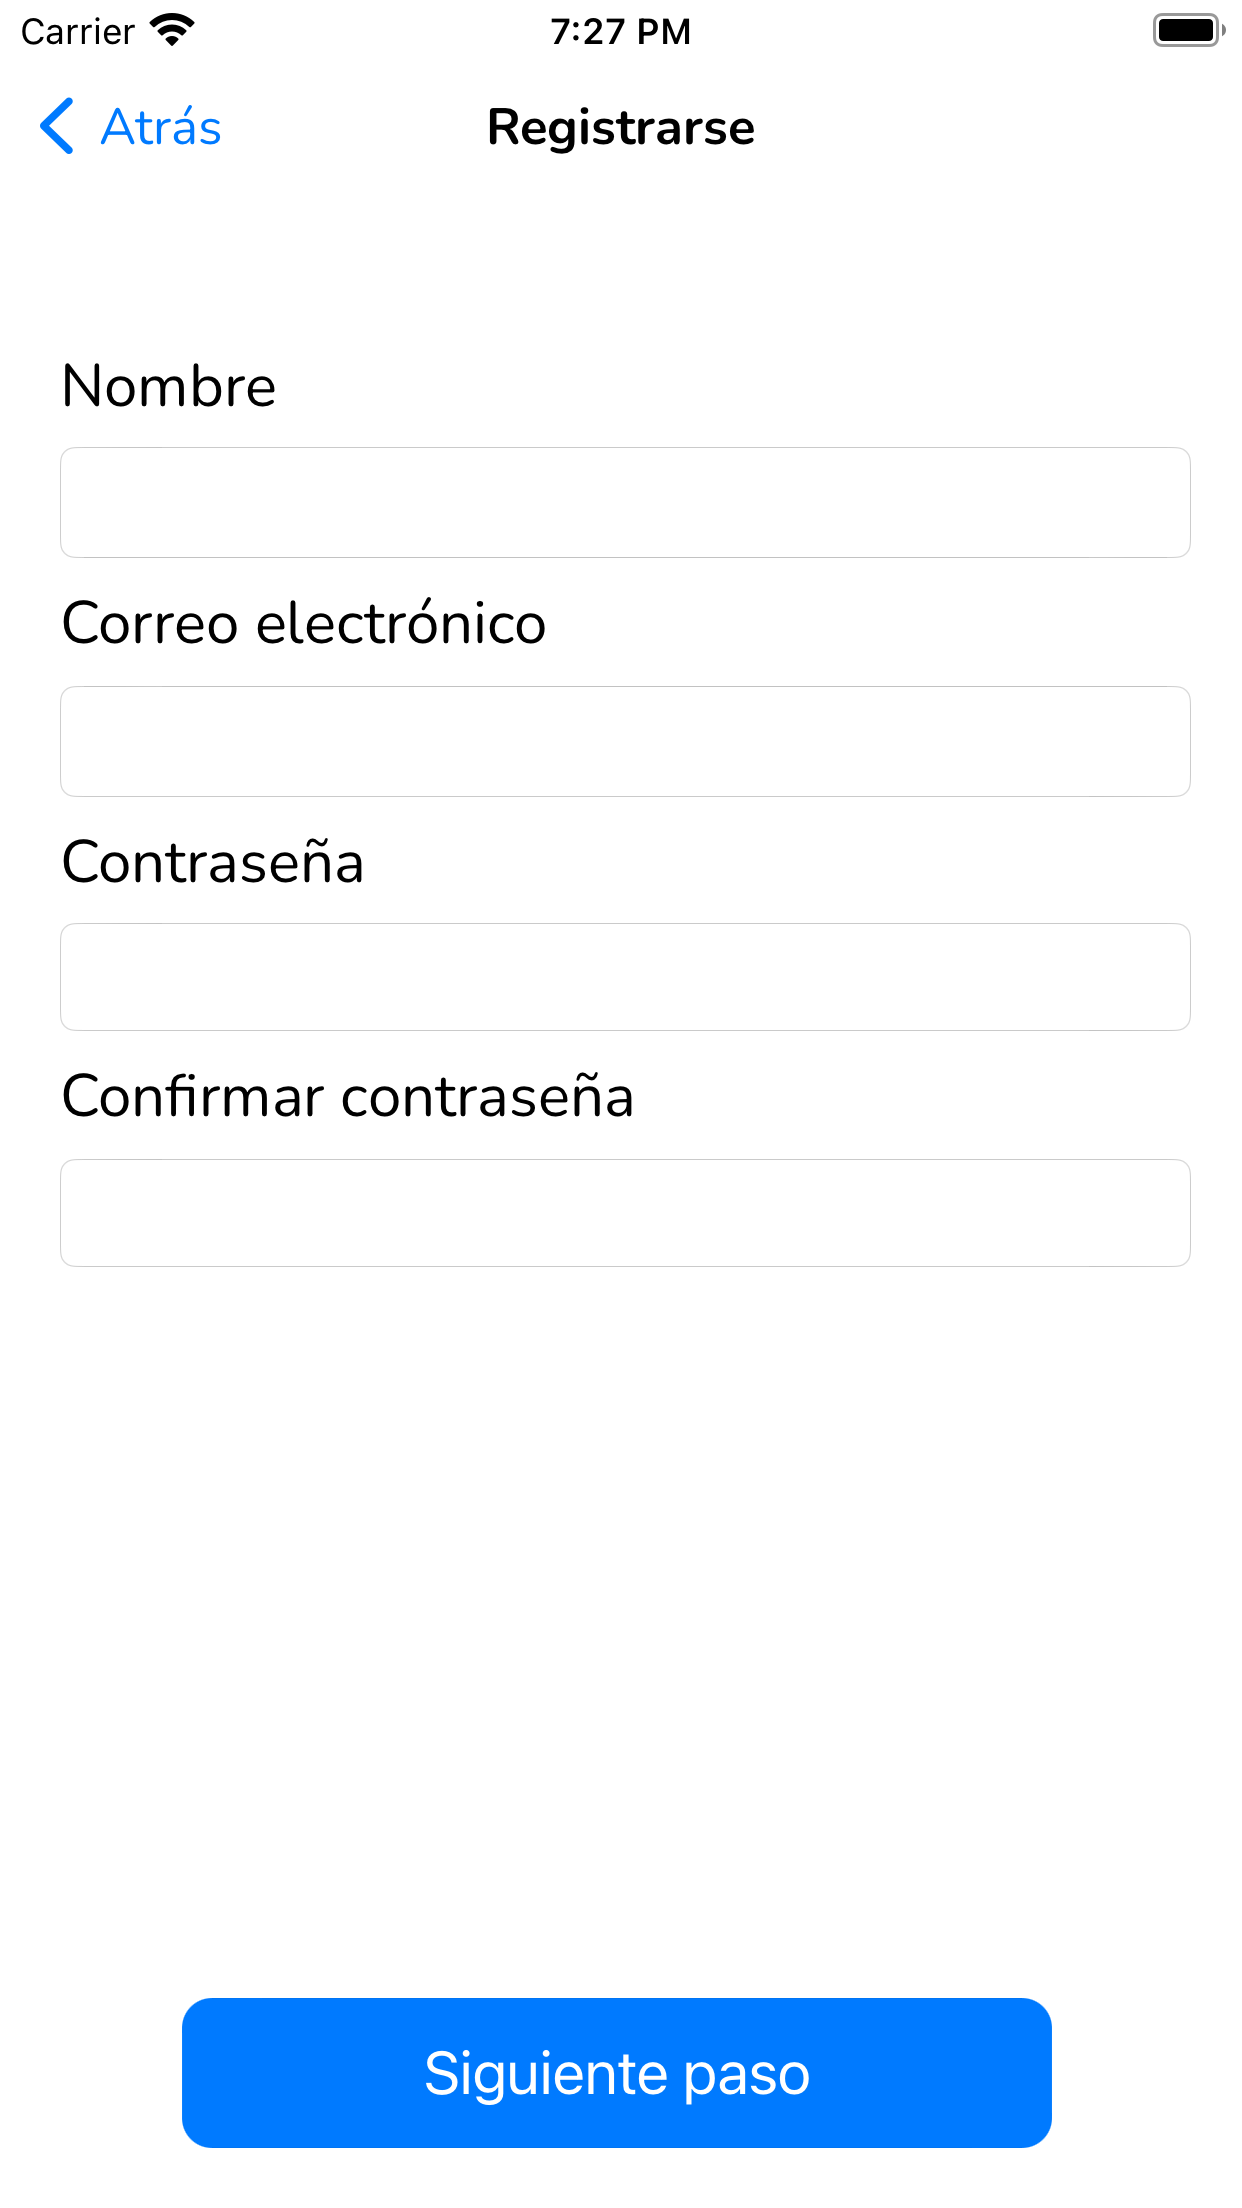
\includegraphics[cframe=black 2pt, width=1\linewidth]{images/manual/registro1.png}
    \end{minipage}
    \begin{minipage}{0.3\textwidth}
        \centering
        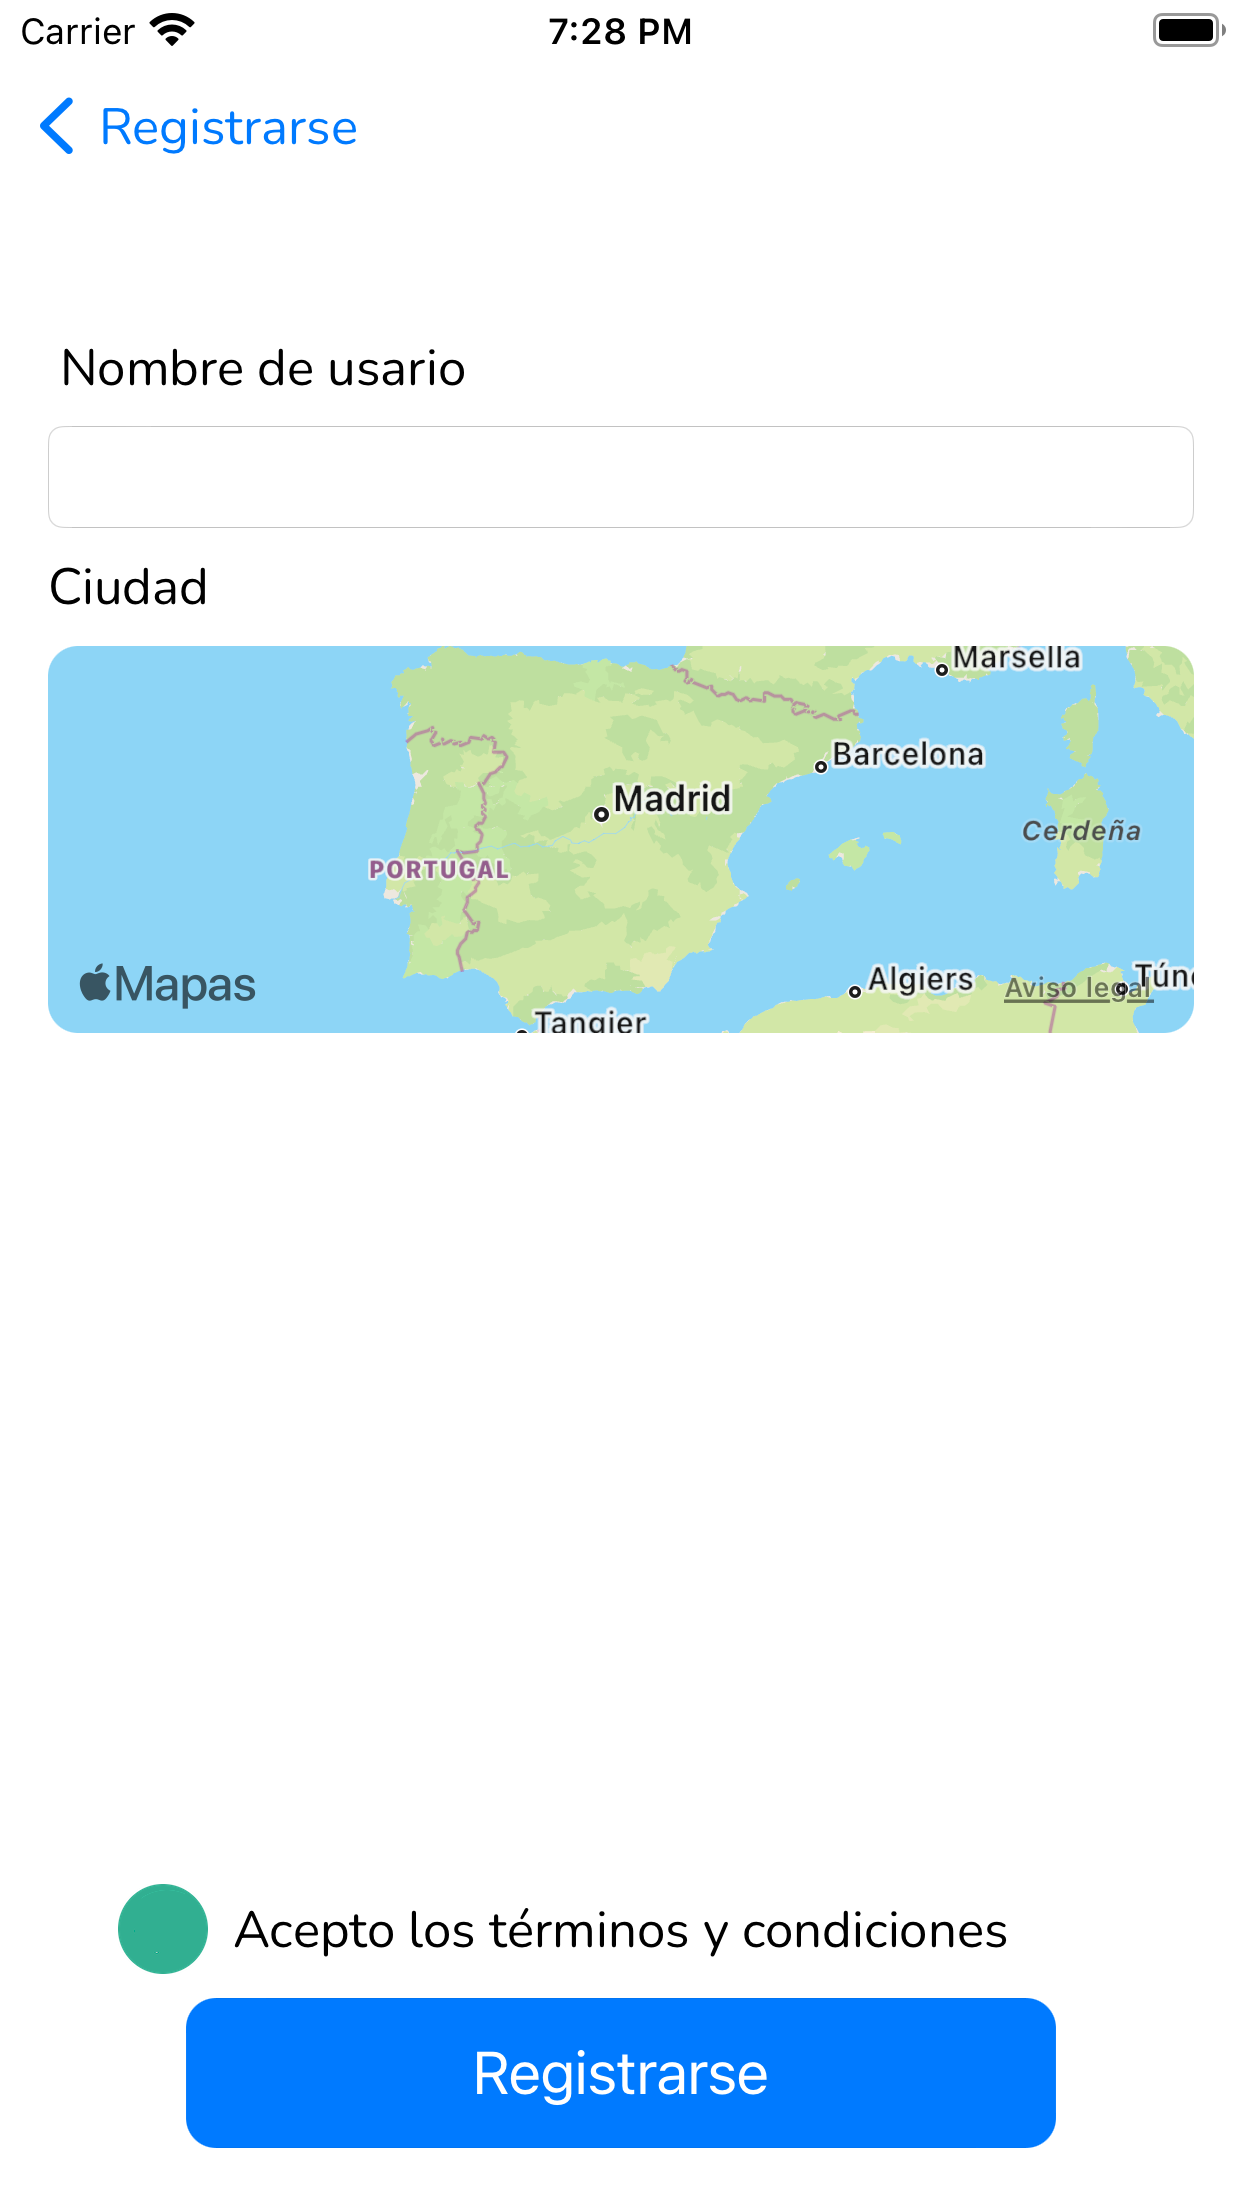
\includegraphics[cframe=black 2pt, width=1\linewidth]{images/manual/registro2.png}
    \end{minipage}
     \begin{minipage}{0.3\textwidth}
        \centering
        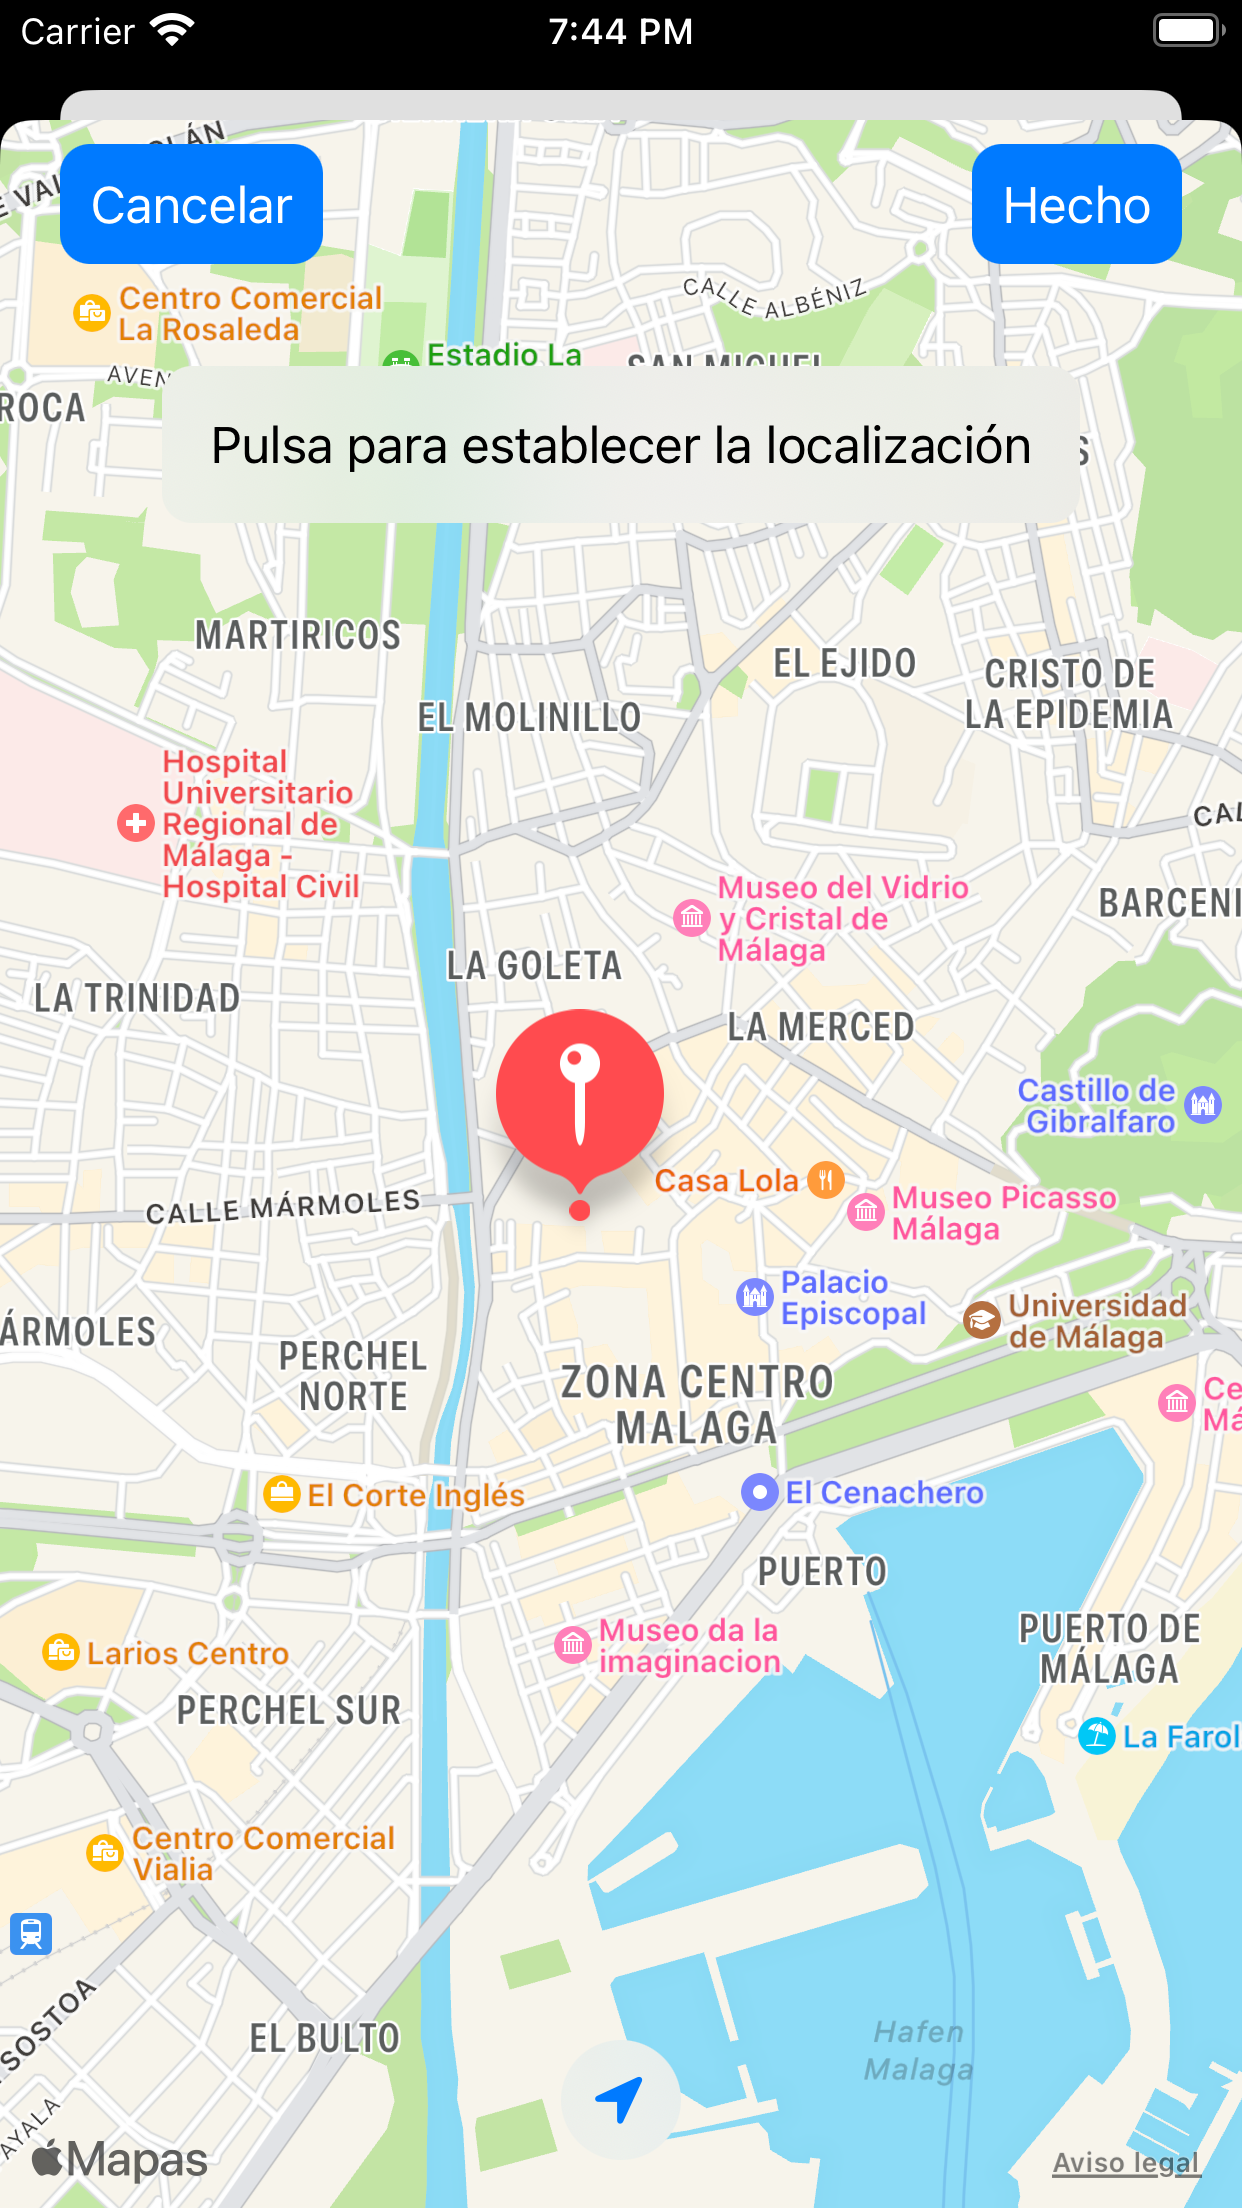
\includegraphics[cframe=black 2pt, width=1\linewidth]{images/manual/mapPicker.png}
    \end{minipage}
    \begin{minipage}{0.3\textwidth}
        \centering
        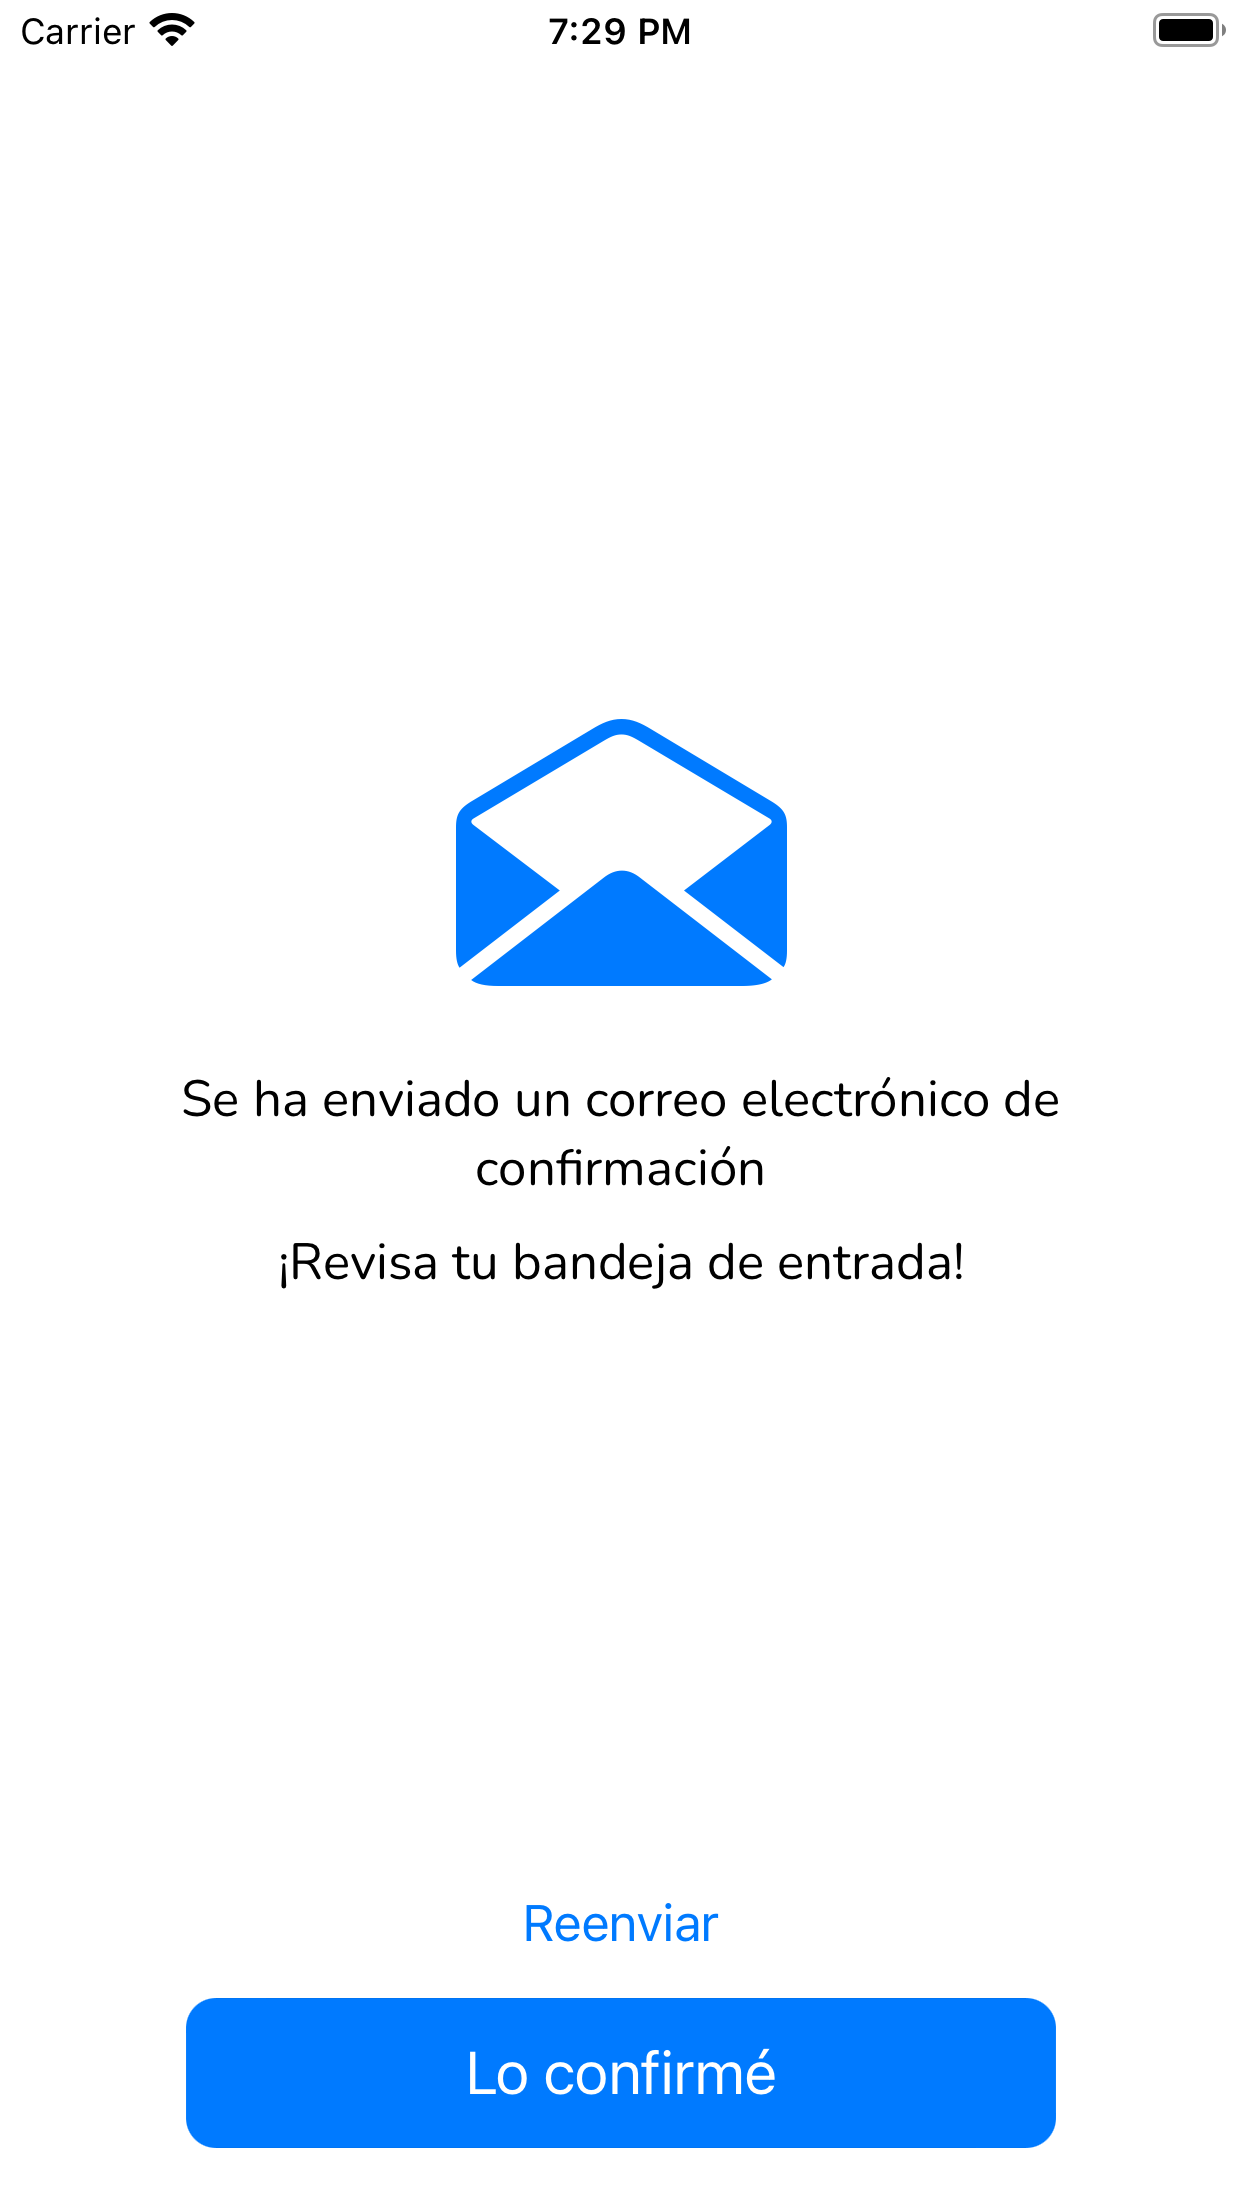
\includegraphics[cframe=black 2pt, width=1\linewidth]{images/manual/registroConfirmacion.png}
    \end{minipage}
    \caption{Login and Register}
    \label{fig:login_register}
\end{figure}
\section{Iniciar sesión}
Para iniciar sesión simplemente el usuario debe proporcionar las credenciales que uso durante el proceso de registro.
\begin{figure}[H]
        \centering
        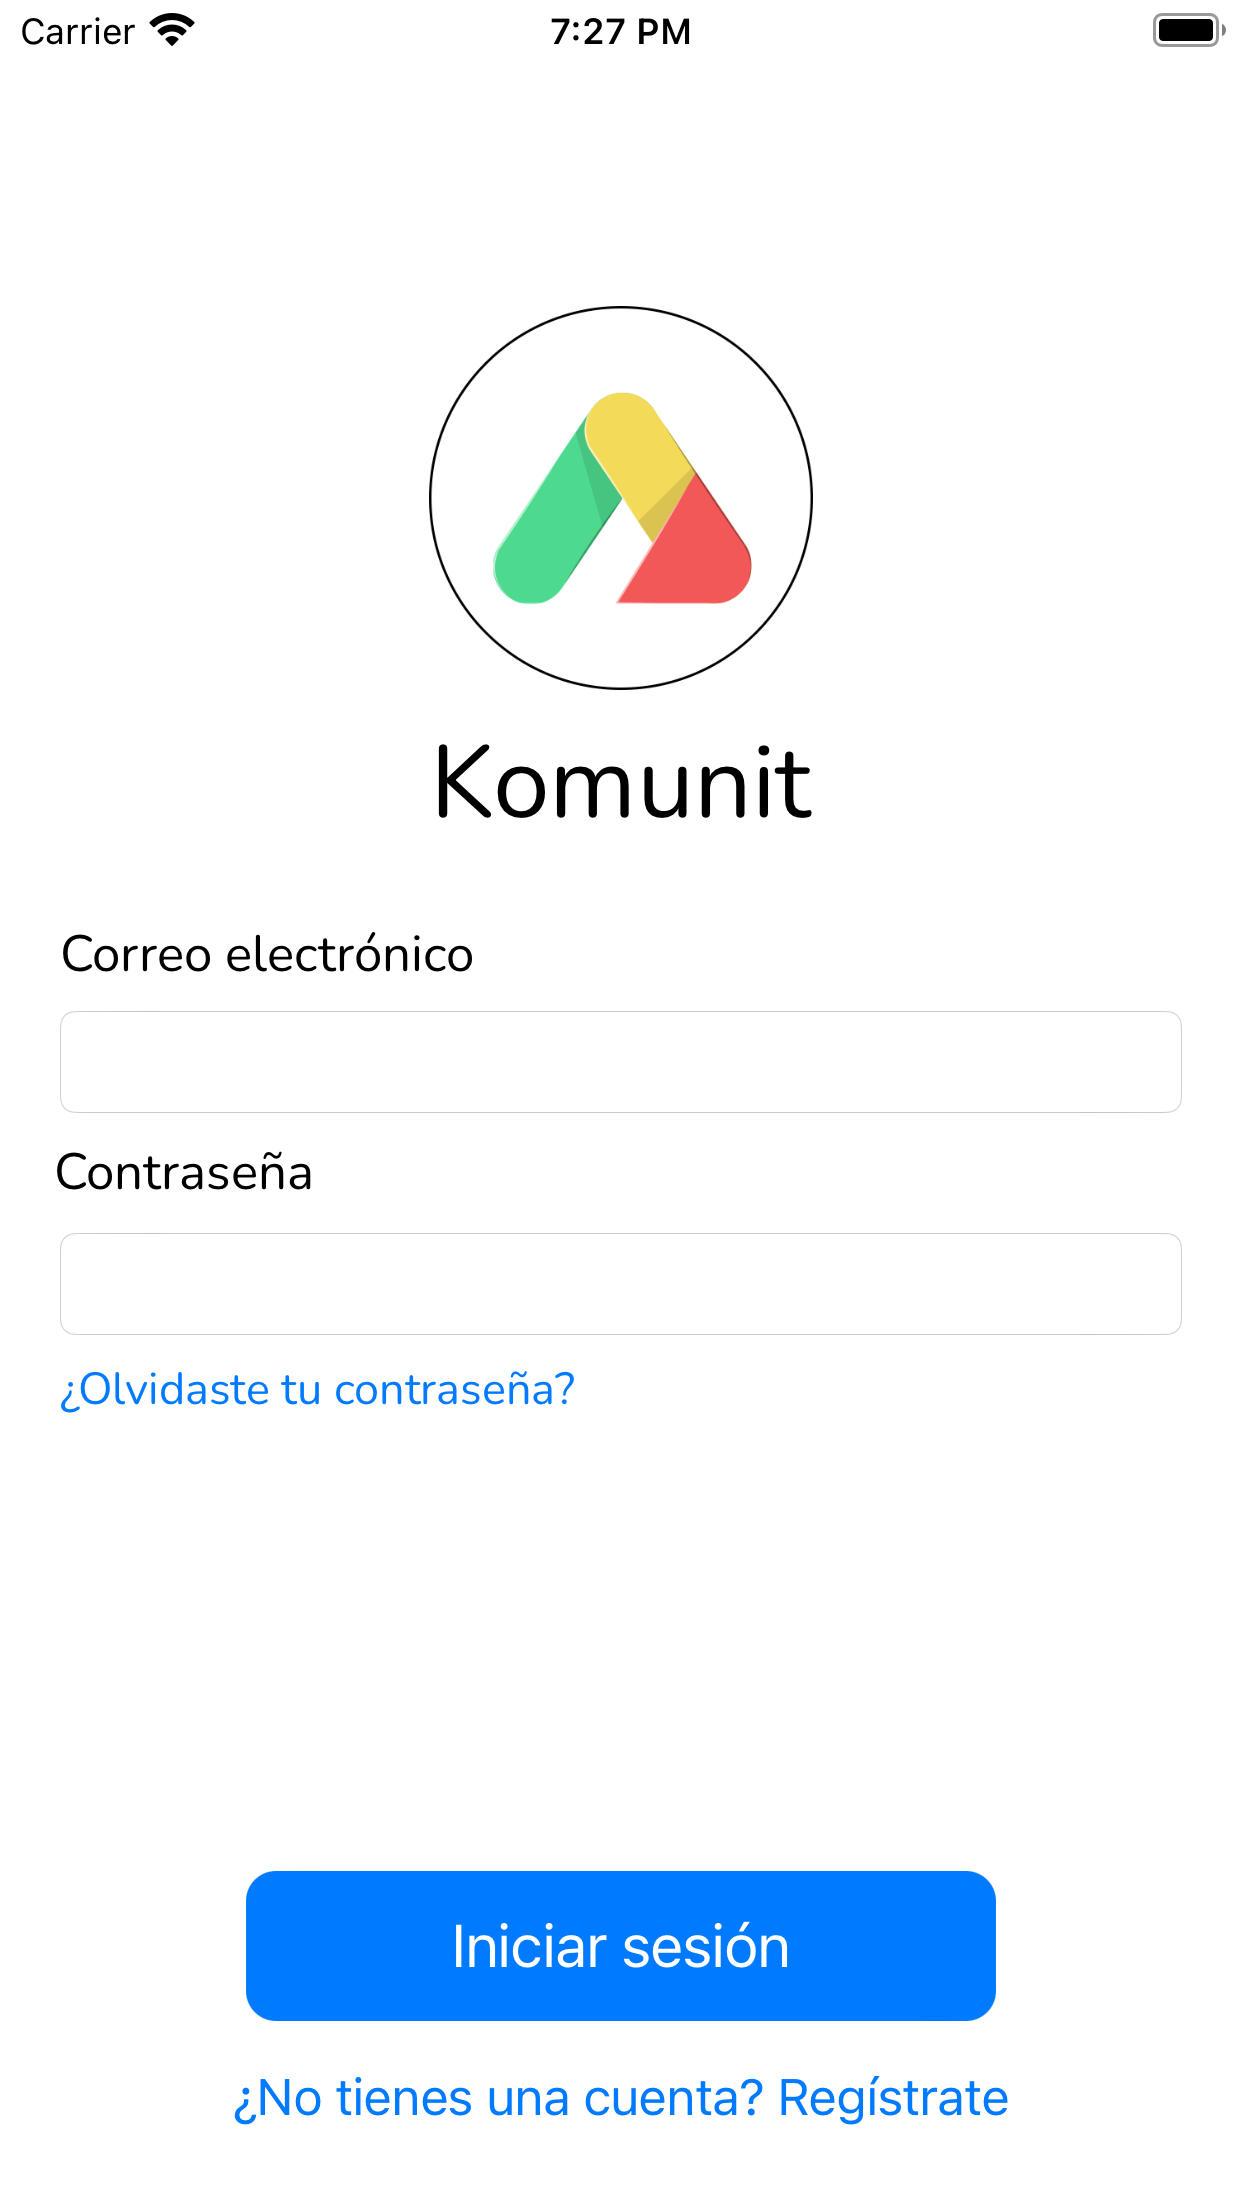
\includegraphics[cframe=black 2pt,width=0.3\linewidth]{images/manual/login.png}
        \caption{Iniciar sesión}
        \label{fig:my_label}
\end{figure}
Después de rellenar correo y contraseña el usuario deberá pulsar el botón ``Iniciar sesión'', si las credenciales son correctas la aplicación redirigirá al usuario a la pantalla principal.

\section{Unirse a un grupo}
Estando en la pantalla principal, el usuario puede explorar grupos alrededor de su localización a través de un mapa interactivo.
\begin{figure}[H]
        \centering
        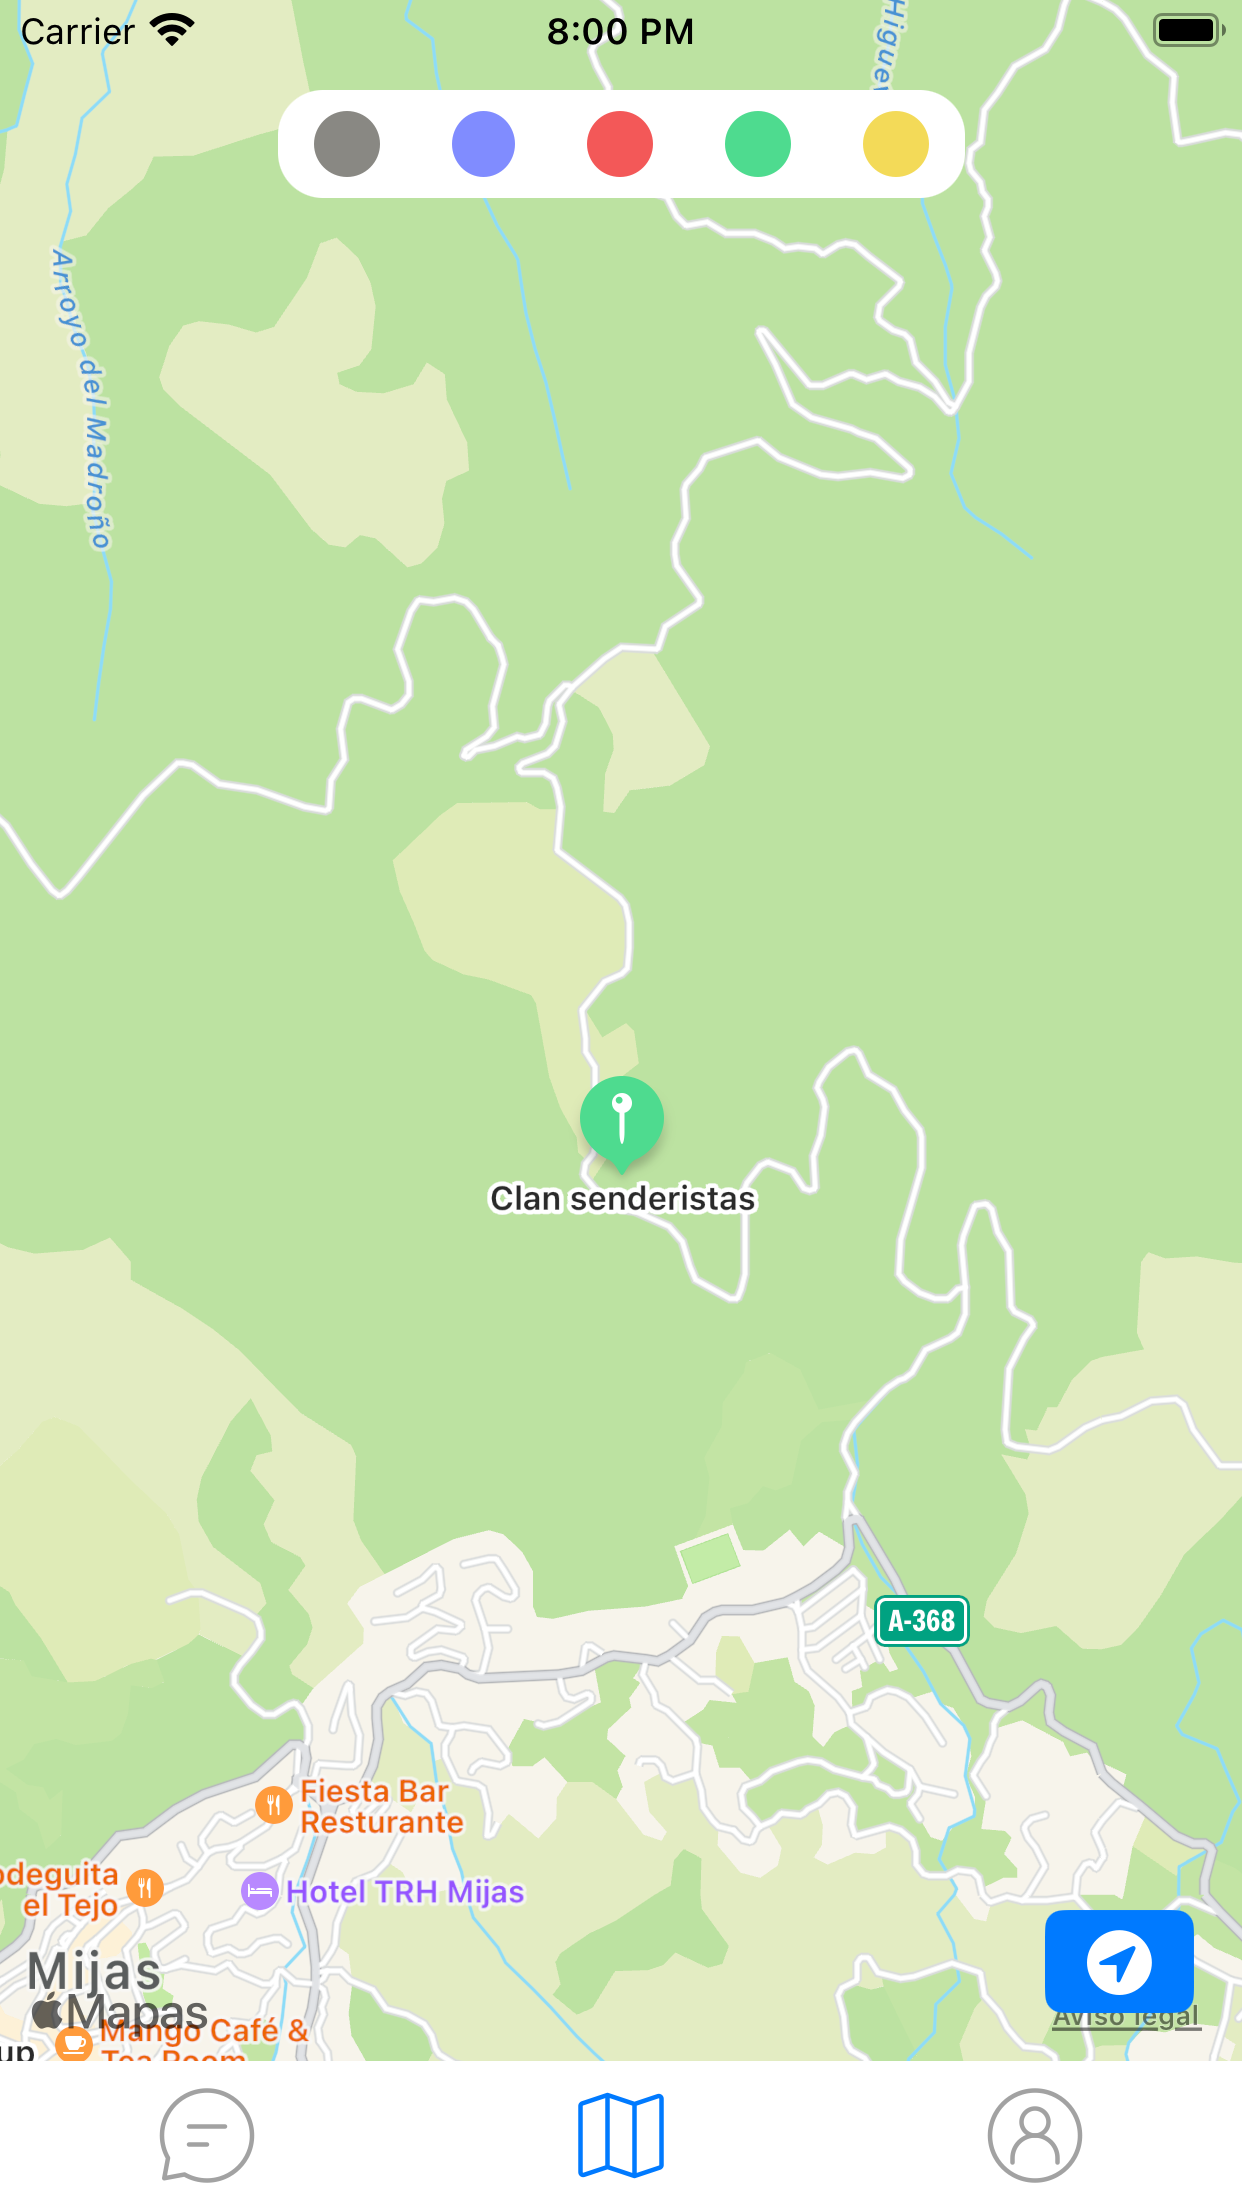
\includegraphics[cframe=black 2pt,width=0.3\linewidth]{images/manual/explorarGruposMapap.png}
        \caption{Iniciar sesión}
        \label{fig:my_label}
\end{figure}
Pinchando sobre el grupo el usuario podrá visualizar una vista detallada de la información del grupo como título, descripción e integrantes. Para unirse a un grupo habrá que pulsar sobre el botón ``Unirse''.

\section{Chatear}
Para acceder al chat de un grupo el usuario deberá dirigirse al listado de grupos pulsando en el primer icono del menú inferior de navegación.
De esta forma podrá visualizar los grupos a los que pertenece ordenados por fecha del último mensaje.
\begin{figure}[H]
        \centering
        \begin{minipage}{0.3\textwidth}
            \centering
            \includegraphics[cframe=black 2pt,width=1\linewidth]{images/manual/listadoGruposChat.png}
        \end{minipage}
        \begin{minipage}{0.3\textwidth}
            \centering
            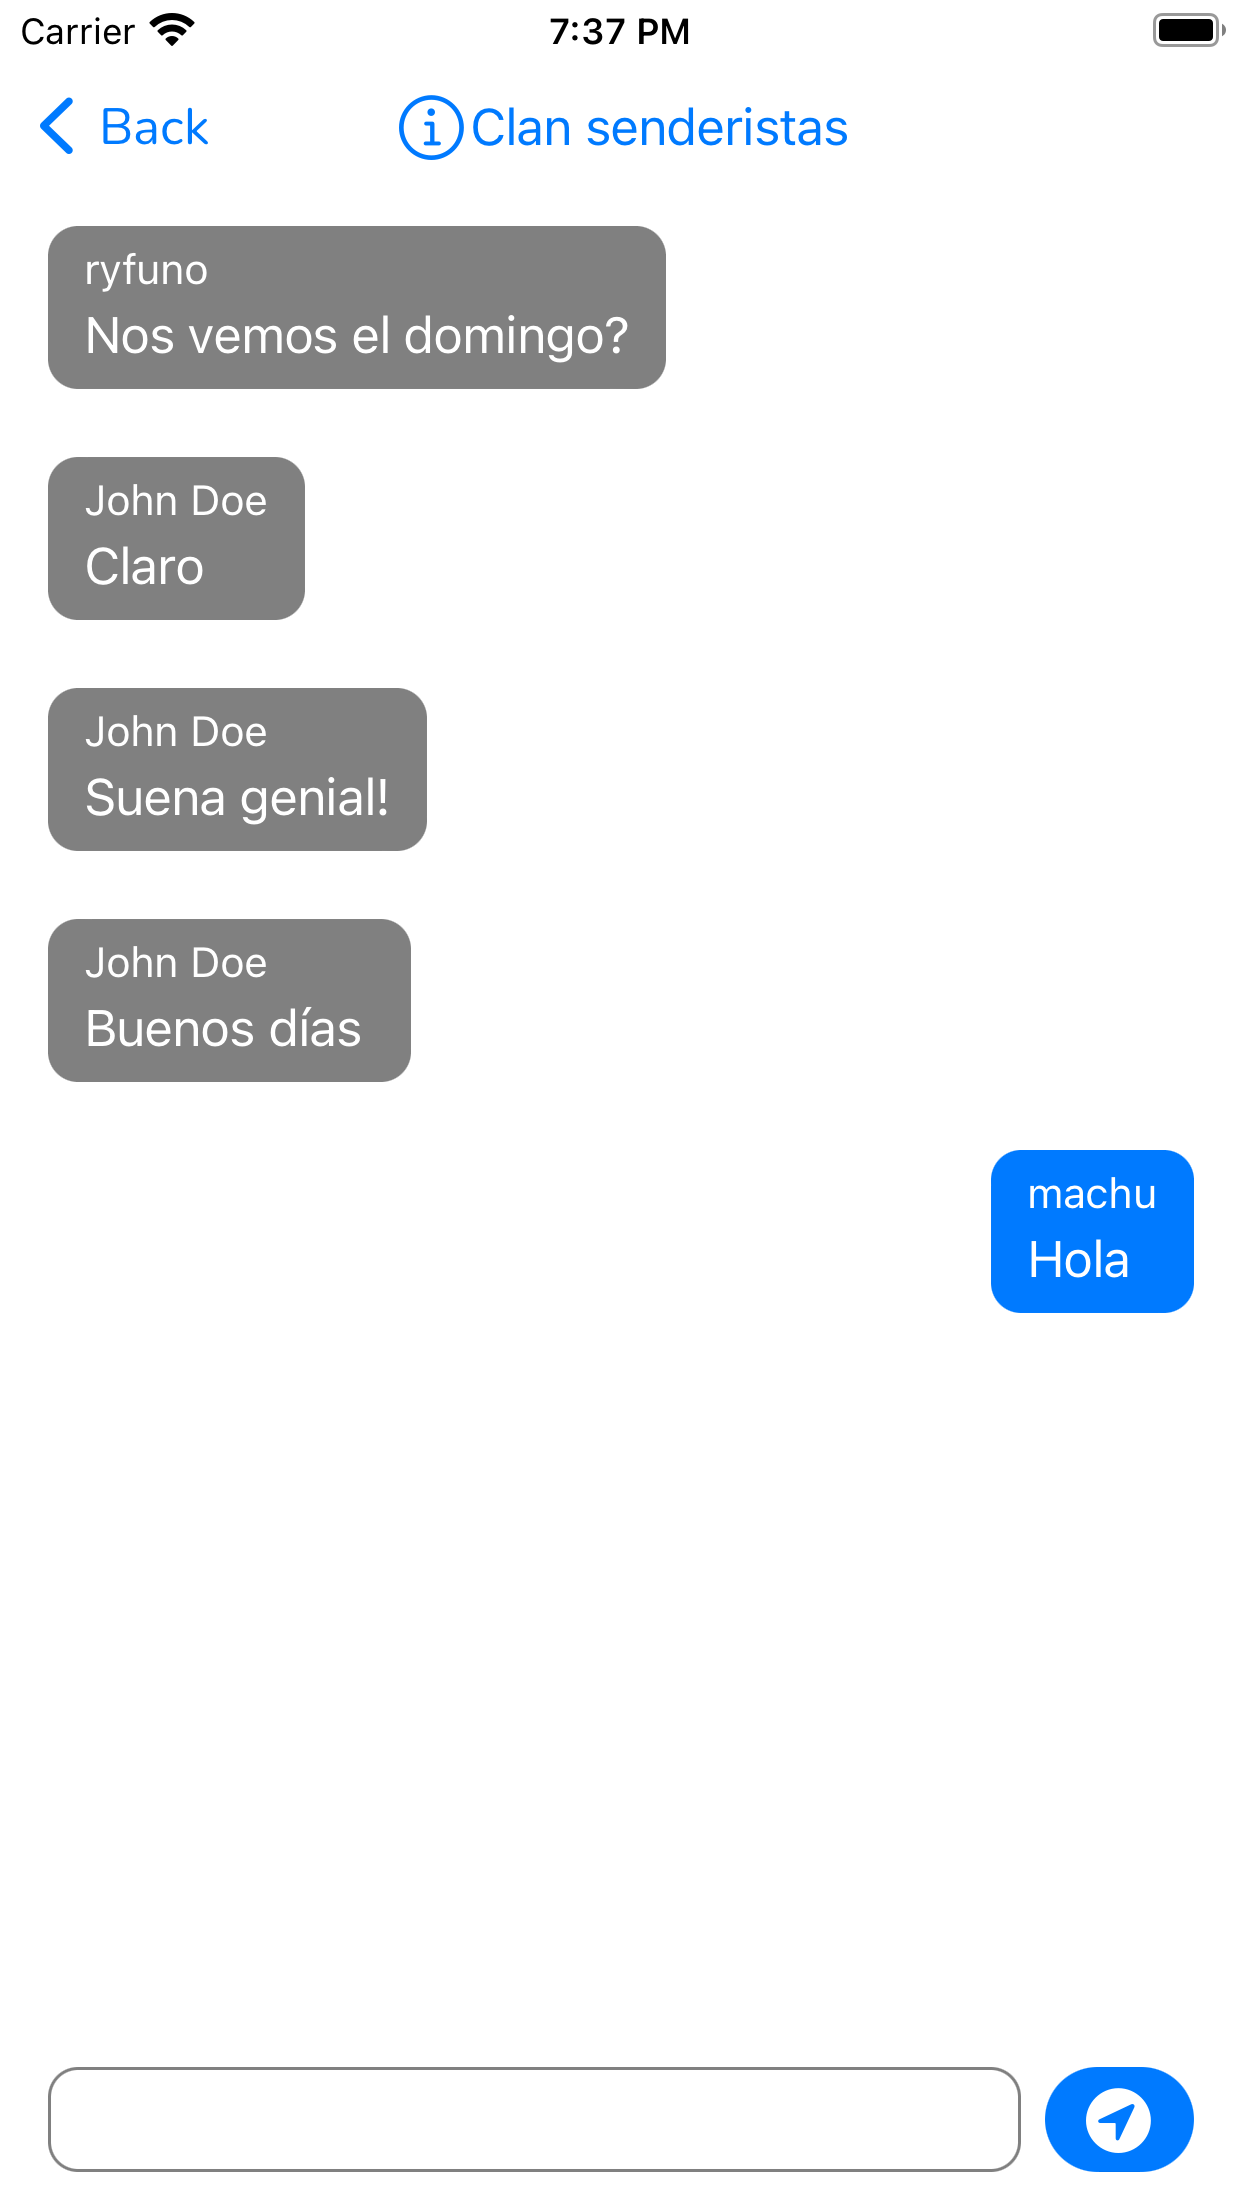
\includegraphics[cframe=black 2pt,width=1\linewidth]{images/manual/ejemploChat.png}
        \end{minipage}
        \caption{Chat}
        \label{fig:my_label}
\end{figure}
\end{appendices}